Les différents services proposés de l'hôpital (pour la gestion des ressources) sont illustrés sur la figure \ref{hopital}.
\newline
\begin{figure}[h!]
	\hspace*{-2.5cm}
	\centering
	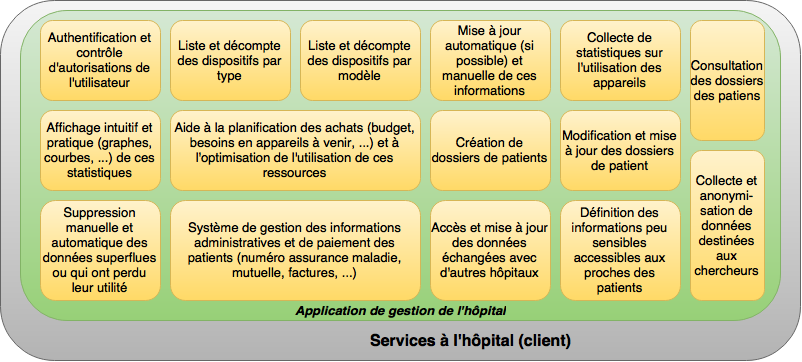
\includegraphics[width=1.4\textwidth]{hopital.png}
	\caption{Services de la Couche Applicative du côté de l'Hôpital}
	\label{hopital}
\end{figure}

La gestion des ressources est une discipline présente dans tous les domaines. Le domaine médical ne fait pas exception à cette
règle. En effet, un certain équipement est nécessaire pour traiter les malades. Ce matériel peut se dégrader avec le temps ou
suite à un accident. A terme il faudra donc le remplacer. Afin de procéder aux achats, il est préférable de faire un inventaire,
cela permet de faire des commandes globales et donc d'économiser de l'argent. De nombreux commerces ferment durant un inventaire
afin de simplifier l'opération, toutefois cette solution n'est pas envisageable dans le cas des hôpitaux en général, en
particulier cela serait inacceptable dans le service des urgences.  
\newline

Le système doit donc permettre de faire un inventaire. Il serait préférable qu'il permette non seulement de connaître le nombre de
dispositifs selon le type de ces derniers, mais aussi le nombre de dispositifs d'un certain modèle. En effet, un modèle pourrait
posséder plus de fonctionnalités, ce qui le rendrait indispensable pour certaines situations, ou du moins plus pratique. Intégrer
cette fonctionnalité à notre système plutôt que de se basé sur un logiciel/mécanisme déjà existant a quelques avantages non
négligeables. En particulier, sous l'hypothèse que chaque capteur possède un trait unique, il est possible d'automatiser une
partie du processus. Comme exemple de trait distinctif, on peut penser aux adresses mac que des constructeurs donnent à leurs
produits. Le principe de fonctionnement serait le suivant: lorsque le capteur se déclare à son moniteur, ce dernier informerait le
système (via un message à la passerelle intelligente) de la connexion qui vient de s'établir. La passerelle pourrait alors
informer un serveur interne qu'un capteur ayant un tel id vient d'initier une connexion. Le système vérifie s'il connaît cet id,
si ce n'est pas le cas il envoie un message à la passerelle demandant plus d'information. Il sera alors de la responsabilité de la
passerelle de le renseigner.  
\newline

Par ailleurs,en plus de connaître le nombre d'appareils, il peut être utile de pouvoir tracer des courbes récapitulant
l'utilisation par type d'appareil. En effet, la possibilité de calculer diverses statistiques permettrait de mieux anticiper les
besoins. En outre, cela est indispensable pour la prise de décision. En l'absence de telles statistiques, il est difficile de
décider le nombre d'appareils à acheter.  
\newline

En plus de pouvoir gérer les ressources, l'hôpital doit également gérer les patients. L'administration doit pouvoir créer un
nouveau dossier pour le patient ou ouvrir un dossier existant. Les informations présentes dans ces dossiers doivent pouvoir être
modifiées, complétées et sauvegardées. Certaines informations perdent de la valeur avec le temps, connaître la température dans
une chambre il y un an a peu d'intérêt. De même connaître l'intégralité des relevés cardiaques un an après n'est pas pertinent.En
plus de pouvoir supprimer des informations manuellement, il est nécessaire de pouvoir le faire de manière automatique pour
certaines données. De plus, conserver un dossier trop longtemps n'est pas nécessairement utile. Il est donc souhaitable que au
bout d'un certain temps ceux-ci soient supprimés automatiquement. Cela permettrait d'éviter la saturation de l'espace de stockage.
\newline

Par ailleurs, un système de gestion de paiement serait utile. Retenir le numéro de sécurité sociale, l'identifiant de la mutuelle
du patient et le statut de paiement serait particulièrement utile. Dans le premier cas, cela permettrait de facturer directement
les organismes payeurs sans avoir à déranger le patient ou la famille. Dans le second cas, cela permettrait de connaître les
patients ne s'étant pas acquittés de leur dû. Et de le leur rappeler si besoin est.
\newline

La présence d'un cloud (public ou privé) impose de pouvoir lire et écrire dessus. Le cloud privé servira de sauvegarde pour les
données du stockage interne. Il est donc important que ces données soient copiées à intervalles réguliers. Le cloud public, lui
contiendra des données anonymisées mises à disposition d'universités ou d'organismes de recherche pour mener à bien des études.
Ainsi que des informations peu sensibles destinées à la famille du patient. Ce cloud public sera également chargé de faire tourner
les différents programmes d'interaction destinés à la famille du patient. Il sera aussi le lieu d'échange de données entre
hôpitaix partenires. Losqu'un hôpital partenaire en fait la demande, il doit pouvoir recevoir les inforamtions d'un ancien patient
de l'hôpital. Ce système d'entre-aide est destiné à permettre aux médecins de prende une décision éclairée en ayant le plus
d'éléments à leur disposition. A l'inverse, l'hôpital peut demander à un partenaire des inforamtions relatives à un patient. Ces
échanges seront sécurisés.
\newline

Bien sûr, l'accès à ces fonctionnalités doit être surveillé et sécurisé. De manière grossière, on peut résumer les différentes
fonctionnalités du présent module de la manière suivante.
\begin{enumerate}
    \item gestion des informations dans le cloud
    \item gestion des informations stockées en interne
    \item gestion du cycle de vie des informations stockées
    \item sécurisation de l'accès aux données (que ce soit en lecture ou en écriture)
\end{enumerate}
